\chapter{Time Normalized Term Weighting}
In this chapter, we introduce the novel algorithm of this research, that is time normalized term weighting. In the standard term weighting methodologies, the terms are weighted based on their spatial distribution rather than on the other crucial factors. Consider an example of two terms "COVID19" and "neural networks". Both the terms represent very different meaning and have a different origin year. "COVID19" is a relatively new term being used since last year, while "neural network" is being used since decades. However, term weighting schemes will weight the terms based only on their frequency distribution, no matter what. In this paper, we try to emphasize on the importance of term recency in relevant results retrieval. The premise for this algorithm is that, if a term is devised newly then there are probably a lesser number of documents containing the term compared to the term which is being used for a longer duration of time. Considering both the aspects of origin year and document frequency, in this algorithm, we introduce a term recency factor along with standard metrics to compute the term weight. The formulation and implementation of the algorithm is further explained in this chapter.

We have also presented this novel algorithm at the WOSP workshop \footnote{WOSP 2020: https://wosp.core.ac.uk/jcdl2020/index.html}, and will be published in the proceedings of the conference. This serves as a contribution to the research community to use this algorithm and can also be extended for further research.

\section{Term Age Calculation}
The time based factor(can also be referred as Term age) is formulated from the origin year of the word(can be from different sources) and the document frequency of the term, computed as the ratio of both giving the metric as documents per year. For a given term $w$ in document $d  \epsilon D$, where $D$  is the document corpus $D$ with size $N$, term-age is calculated as:
\begin{equation}
    t_{w,D}=\log(df_{w,D}/(y_{diff}+1))
\end{equation}
where $y_{diff}$ is calculated as :
\begin{equation}
    y_{diff} = y_{current} - y_{origin}
\end{equation}
where $y_{origin}$ is the year of first usage of the word and $Y_{current}$ is the present year.

We have not considered the article publishing year and take current year for certain reasons. Since a term can be used in multiple years, so the age calculation would change every time and choosing either of them would be a tough call. Also, this might result in certain anomalies and ambiguities in the age calculation. To simplify this logic and to have the same age for a term across the corpus, we consider the current year, which is the last year of articles published in the corpus. We take the logarithm of the terms to normalize the value, since this can go to a large number based on the size of the corpus. Also, we take up the absolute value of log, so that we don’t have negative weight values. 1 is added in the denominator to avoid the divide by zero error in case if the origin year is same as the current year. 

The $y_{origin}$ can be traced from multiple sources depending on the problem statement. Considering few examples, and the formulation of term age factor respectively:
\begin{itemize}
    \item if a research paper recommender is being developed, the origin year can be retrieved from the year of first occurrence in a research paper. And the current year can be the last year of the article/paper present in the corpus.
    \item in case of web based personalized search engine, time of first search of the specific term can be used to form the temporal context as used in \cite{RN27}. The difference from the first usage year to the current year can be used as the year difference.
    \item for a more generic instances and to make the calculation more robust, the origin year can be traced to the etymology and the year of first occurrence can be fetched. This can also be used to fetch other contexts of the word based on the word origin, and usage to improve search results and recommendations however, these aspects are beyond the scope of this research.
\end{itemize}
In our research hypothesis, we have used the origin year as the generic one and fetch it from etymonline.com to get the etymology and fetch the year of first occurrence. We have used the news dataset \cite{RN20}, that have terms being used which explain a wide range of temporal context. We have also tested the same algorithm on research paper dataset \cite{DBLP:conf/ijcai/WangCL13} and a web answer retrieval dataset \cite{RN30, RN31}. And also to keep the algorithm more robust and generic, testing the etymology seems to be an apt way to test the hypothesis. We have introduced the term age factor in three of the term weighting schemes, that is TF-IDF, BM25 and USE, explained in the following sections.


\section{Time Normalized TF-IDF(tTF-IDF)}
TF-IDF is the classic term weighting methodology, that weights the terms based on two factors, term frequency and inverse document frequency. Both these factors are based on the spatial distribution of terms that is the frequency of their occurrence in the corpus. This formulation is shown in Equation \ref{eq:4.3}
\begin{equation} \label{eq:4.3}
        wt_{w,d} = tf_{w,d}*log(\frac{N}{df_{w,d}})   
\end{equation} 
The real issue in this formulation is that, the TF-IDF assumes that a frequency distribution remains constant over time. In short periods of time, this holds true, however, over longer periods of time, this assumption fails. To overcome the issue that terms have temporal distributions of frequency not just space distribution, which are unaccounted when using TF-IDF, we proposee the time normalized TF-IDF. This is computed as shown in equation \ref{eq:4.4}.

\begin{equation} \label{eq:4.4}
        wt_{w,d} = t_{w,D}*tf_{w,d}*log(\frac{N}{df_{w,d}})   
\end{equation} 

With the introduction of term age factor, we intend to incorporate the temporal context of the terms for an improved search results.

\begin{figure}
    \centering
    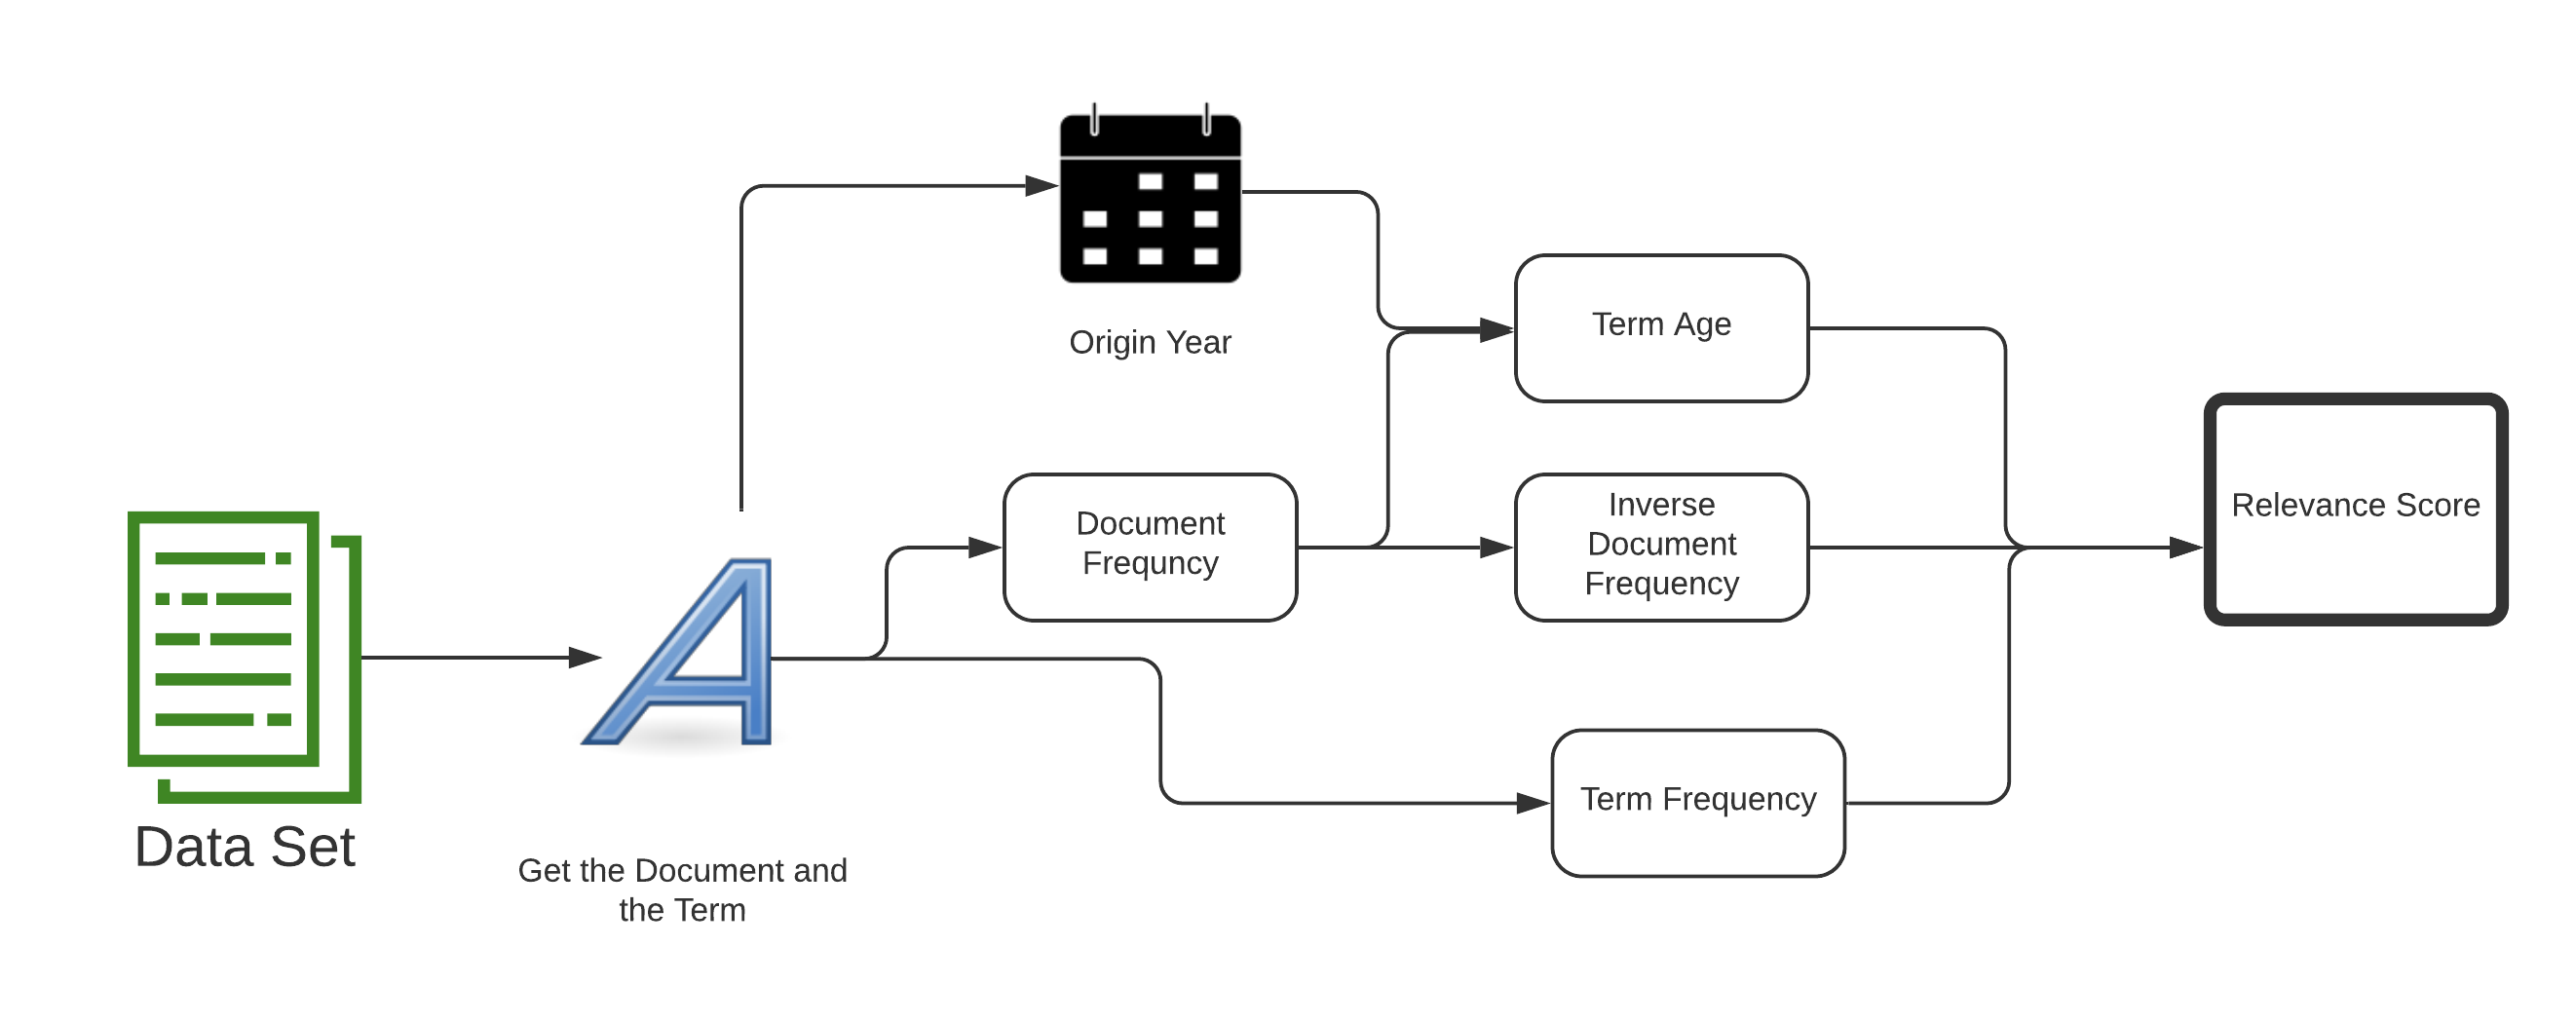
\includegraphics[width=\textwidth] {algorithm-working.png}
    \caption{Algorithm Working for tTF-IDF }
    \label{fig:tTF-IDF-working}
\end{figure}

\section{Time Normalized BM25(tBM-25)}
BM25 is another standard term weighting methodology that is also based on term frequency and inverse document frequency calculations, but the logic to calculate these metrics changes. IDF is calculated the same way as in the TF-IDF but with an added 1 in the denominator to overcome the divide by zero error. For computing the term frequency, some additional term based metrics such as field length and average field length are considered. Some other constants such as k1 and b are also considered in this formula, that are used to normalize the term weighting scores. This formulation is shown in Equation \ref{eq:4.5}.
\begin{equation}  \label{eq:4.5}
    wt_{w,d} = \sum_{i}^{n}IDF(q_{i}) * \frac{f(q_{i},D)*(k1+1)}{f(q_{i},D)+k1*(1-b+b*\frac{fieldLen}{avgFieldLen})}
\end{equation}
Although this overcomes the issues found in the TF-IDF and performs better in some cases, but the issue of not considering the diverse context of the term in various aspects still remains the same. Even the added metrics such as field length and constants k1 and b, are all based on the spatial distribution of the terms. As we formulate the tTF-IDF, similarly, we deduce the formula for tBM25 introducing the term age in the term weight calculation. This formulation is shown in Equation \ref{eq:4.6}. And this time-normalized term age factor works on to consider the temporal aspect of the terms as well.
\begin{equation}  \label{eq:4.6}
    wt_{w,d} = \sum_{i}^{n} t_{w,D}*IDF(q_{i}) * \frac{f(q_{i},D)*(k1+1)}{f(q_{i},D)+k1*(1-b+b*\frac{fieldLen}{avgFieldLen})}
\end{equation}
\section{Time Normalized USE(tUSE)}
Universal Sentence Encoder(USE) is not specifically a term weighting methodology but a more advanced scheme. Text embedding and sentence embedding model convert the given text into high dimensional vectors and then the similarity between these vectors is mostly calculated using the cosine similarity function. This cosine similarity finds the angle between the given vectors and the lesser the value of the angle, more similar the texts are. This formula for finding the cosine similarity between the high dimensional vectors is given in Equation \ref{eq:4.7}.
\begin{equation} \label{eq:4.7}
    \cos \theta = \frac{\sum_{1}^{n} \vec a_{i}b_{i}}{\sqrt{\sum_{1}^{n} \vec a_{i}^2}\sqrt{\sum_{1}^{n} \vec b_{i}^2}}
\end{equation}
The main advantage of using the USE model in the text retrieval task is that it considers the semantic context of the text along with frequency distribution. This performs well in most of the text based searches and gives pretty good results in our datasets as well. However, the issue we are addressing in this research still remains missing in the formula logic. Similar to other two term weighting methodologies, we have multiplied the term age factor with the regular cosine similarity function for text similarity and get the updated version as tUSE. This computation is shown in equation \ref{eq:4.8}.
\begin{equation} \label{eq:4.8}
    \cos \theta = t_{w,D}*\frac{\sum_{1}^{n} \vec a_{i}b_{i}}{\sqrt{\sum_{1}^{n} \vec a_{i}^2}\sqrt{\sum_{1}^{n} \vec b_{i}^2}}
\end{equation}
\section{Algorithm Analysis}
As we can see the term age is not only dependent on the origin year but also the number of documents the term occurs in(document frequency). This can also be considered as an added factor to the IDF value, but with a different significance. Let us consider the impact that document frequency and time difference have on the term weight value. Now, assume that a term is new and occurs in reasonable number of documents, then the value of term-age, $t_{w,D}$ will be large and hence the term weight will be large.
And contrast case if the term is relatively new, and occurs is lesser number of documents, that is an expected behaviour that the term would be weighted low due to its lesser significance value.
Similarly, if the term is being used for many years and is occurring in many documents, it will relatively reduce the value of the time-factor, thus giving it low importance. 

A caution which needs to be taken while implementing this algorithm is to check for more commonly occurring non relevant terms which are normalized by using IDF should not get boosted. For example, occurrence of stop words, these occur maximum number of times in any corpus, and are irrelevant in general search retrieval schemes. This can be taken care of while calculating the value of $y_{origin}$, and such terms can be ignored so they don’t boost up the term weights based on non-relevant terms. Or if the stops words don't have much significance even in the semantic logic of the retrieval system, they can be removed in the first index itself. That will save the computation as well as reduce the chances of unwanted partiality in the results.
